\section{Дескриптор признаков Shape Context}
Shape Context --- это название, данное дескриптору признаков Serge Belongie и Jitendra Malik, который впервые представили в~\cite{belongie002}. Shape Context может быть использован в распознавании объектов.

\subsection{Теория}
Shape Context используется для описания форм (\emph{shape}). Он позволяет измерять сходство объектов и получать соостветствия между точками объектов. Основная идея состоит в том, чтобы взять $n$ точек на контуре формы. Для каждой точки $p_i$ на форме есть $n-1$ векторов, полученных соединением точки $p_i$ с остальными точками на контуре. Множество этих векторов является слишком детальным описанием формы в точке $p_i$. Ключевая идея состоит в предположении, что распределение относительных позиций --- достаточно надежный, устойчивый к ошибкам, компактный и очень различающий дескриптор. То есть для точки $p_i$ гистограмма распределения относительных координат остальных $n-1$ точек определена как:
\begin{displaymath}
  h_i(k) = \#\{q \neq p_i : (q - p_i) \in bin(k)\}
\end{displaymath}

$h_i(k)$ -- дескриптор признаков Shape Context для точки $p_i$. Столбцы гистограммы обычно выбираются единообразными в полярных координатах. То, что Shape Context является детальным и в то же время различающим дескпиртором, видно на рис.~\ref{shape-context}, на котором показаны дескрипторы двух различных версий буквы ``А''.

\begin{figure}
  \centering
  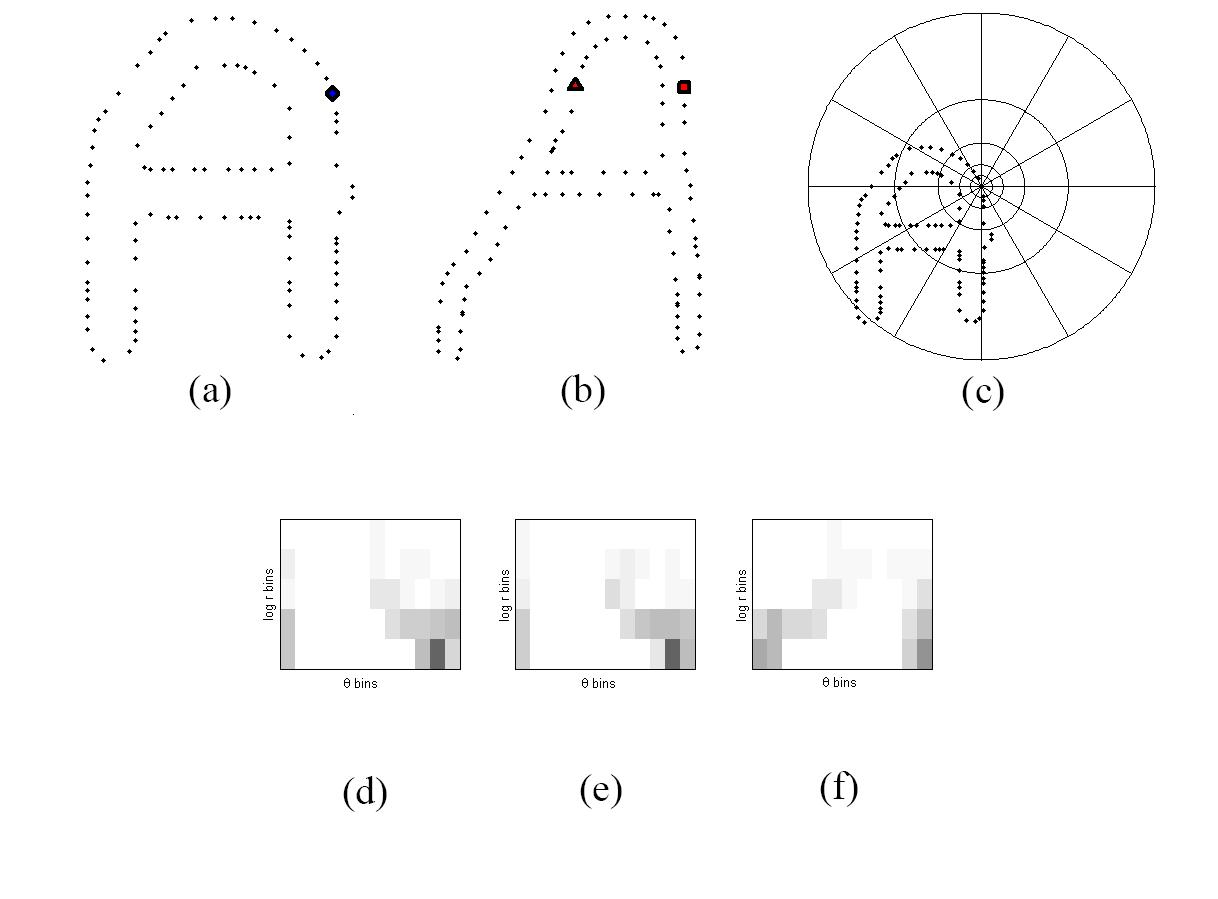
\includegraphics[width=0.9\textwidth]{images/shape-context.png}
  \caption{\label{shape-context}}
\end{figure}

Рис.~\ref{shape-context} (a) и (b) --- точки контура двух форм. Рис.~\ref{shape-context} (c) --- диаграмма столбцов гистограммы в полярных координатах, использованная для подсчета дескриптора. Рис.~\ref{shape-context} (d) --- дескриптор для окружности, (e) --- для ромба и (f) --- для треугольника. Так как (d) и (e) --- дескрипторы для двух точек, которые находятся на очень подобных фигурах, то они очень похожи; в то время как дескриптор (f) сильно отличается.

Чтобы дескриптор признаков можно было применить в реальных задачах, он должен обладать некоторыми инвариантами. Говоря более конкретно, он должен быть инвариантен к параллельному переносу, масштабированию, небольшим возмущениям и --- если того требует задача --- повороту. Инвариантность по отношению к переносу дескриптора очевидна. Инвариантность к масштабированию получается путем деления расстояний между всеми точками на среднее расстояние $\alpha$, хоть медиана распределения расстояний тоже может быть использована.

Также можно получить инвариантность к повороту. Одним из способов является измерение углов в каждой точке, относительных к касательной в той точке (точки выбраны ведь на краях формы). Эта инвариантность не всегда желаема, так как некоторые локальные признаки становятся неразличимыми, если они не зафиксированы в одном и том же положении. В некоторых приложениях вообще избегают инвариантность к повороту, например, в приложении распознавания цифр, чтобы мочь отличать ``6'' от ``9''.

\subsection{Применение в сопоставлении форм}
Приложение, которое использует дескриптор признаков Shape Context, для сопоставления форм состоит из следующих шагов:
\begin{enumerate}
  \item Случайным образом выбрать множество точек, которые лежат на краях известной формы и другой множество точек на неизвестной форме.
  \item Подсчитать дескриптор для каждой точки, найденной на предыдущем этапе.
  \item Сопоставить каждую точку известной формы точке неизвестной формы. Чтобы уменьшить стоимость сопоставления, можно сперва выбрать преобразование (например, аффинное преобразование или thin plate splite, TP-сплайн), которое деформирует известную форму в неизвестную (проще говоря, сравнить две формы). Затем выбрать для каждой точки на неизвестной форме наиболее соответствующую точку на известной.
  \item Подсчитать ``расстояние'' для каждой пары точек двух форм. Для этого использовать взвешенную сумму расстояний, разлечие представлений изображения и энергию, которая необходима для преобразования одной формы в другую.
  \item Чтобы распознать неизвестной формы, использовать классификатор по ближайшему соседу.
\end{enumerate}

\subsection{Детали реализации}
\subsubsection{Поиск точек на краях формы}
Алгоритм предполагает, что форма объекта может быть описана конечным подмножеством точек, лежащих на внутреннем или внешнем контурах. Они могут быть получены с помощью оператора обнаружения краев Канни и последующим случайным выбором из точек, составляющих края. Nota bene: эти точки не должны в общем случае быть ключевыми, например, в местах максимального изгиба края или точками перегиба. Рекомендуется выбирать точки, которые расположены равномерно по контуру, хоть это и не является обязательным.

\subsubsection{Вычисление дескриптора}
Этот шаг рассматривался выше.

\subsubsection{Вычисление матрицы стоимости}
Рассмотрим две точки $p$ и $q$, для которых есть гистограмы из $K$ столбцов $g(k)$ и $h(k)$. Так как дескрипторы --- это распределения, представленные гистограммами, целесообразно использовать критерий согласия Пирсона как стоимость сопоставления двух точек.
\begin{displaymath}
  C_S = \frac{1}{2}\sum_{k = 1}^{K}{\frac{[g(k) - h(k)]^2}{g(k) + h(k)}}.
\end{displaymath}

Результат принадлежит отрезку $[0,1]$. В добавок к этой стоимости, может быть добавлена стоимость, основанная на представлении (\emph{appearance}) изображения. Например, она может быть мерой различия углов к касательной (очень полезна в распознавании цифр):
\begin{displaymath}
  C_A = \frac{1}{2}
  \begin{Vmatrix}
    \dbinom{\cos(\theta_1)}{\sin(\theta_1)} - \dbinom{\cos(\theta_2)}{\sin(\theta_2)}
  \end{Vmatrix}
\end{displaymath}

$C_A$ равно половине длины хорды единичной окружности между единичными векторами с углами $\Theta_1$ и $\Theta_2$. Это значение также принадлежит $[0, 1]$.

Полная стоимость теперь может быть представлена как взвешенная сумма двух вышеприведенных стоимостей:
\begin{displaymath}
  C = (1 - \beta)C_S + \beta C_A.
\end{displaymath}

Теперь для каждой точки $p_i$ первой формы и $q_i$ второй формы подсчитаем стоимость сопоставления и обозначим ее как $C_{ij}$. Итак, матрица стоимостей получена.

\subsubsection{Поиск сопоставления, которое минимизирует общую стоимость}
Теперь следует найти такое сопоставление, которое минимизирует общую стоимость
\begin{displaymath}
  H(\pi) = \sum_i{C(p_i, q_{\pi(i)})}.
\end{displaymath}

\begin{figure}
  \centering
  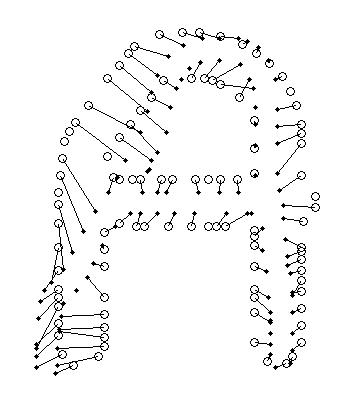
\includegraphics[width=0.4\textwidth]{images/shape-context-matching.png}
  \caption{Результат сопоставления\label{shape-context-matching}}
\end{figure}

Это можно выполнить, исползуя венгерский метод, за время $O(n^3)$.

\subsubsection{Моделирование трансформации}
Получив множество соответствий между точками форм, преобразование $T : \Bbb{R}^2 \to \Bbb{R}^2$, для отображения любой точки первой формы на точки второй формы, может быть смоделировано. Есть несколько моделей, о которых пойдет речь ниже.

\emph{Аффинное преобразование}. Часто выбирают в качестве преобразования афинное преобразование: $T(p) = Ap + o$. Решение для матрицы $A$ может быть получено с помощью метода наименьших квадратов, а вектор переноса следующим образом:
\begin{gather*}
  o = \frac{1}{n}\sum_{i=1}^n \left (p_i - q_{\pi(i)} \right )\\
  A = (Q^+ P)^t,
\end{gather*}
где $P = \begin{pmatrix}
  1 & p_{11} & p_{12} \\
  \vdots & \vdots & \vdots \\
  1 & p_{n1} & p_{n2}
  \end{pmatrix}$, а $Q$ --- по аналогии с $P$. $Q^+$ --- псевдообратная матрица $Q$.

\emph{Thin plate сплайны}. Модель thin plate сплайнов (TPS) наиболее широко применимая модель трансформации при использовании дескриптора признаков Shape Context. Двумерное преобразование может быть представлено двумя TPS-функциями, чтобы смоделировать преобразование координат:
\begin{displaymath}
  T(x,y) = \left (f_x(x,y),f_y(x,y)\right ),
\end{displaymath}
где $f_x$ и $f_y$ имеют следующую форму:
\begin{displaymath}
  f(x,y) = a_1 + a_xx + a_yy + \sum_{i=1}^n\omega_iU\left (\begin{Vmatrix}
    (x_i,y_i) - (x,y) \end{Vmatrix} \right ),
\end{displaymath}
где $U(r)$ --- ядро, определенное как $r^2\log r^2$. Детали о том, как получить решение, могут быть найдены в \cite{powell95} и \cite{duchon}.

\subsubsection{Вычисление расстояние между формами}
Расстояние между формами $P$ и $Q$ будет взвешенной суммой трех слагаемых (не все они обязательно должны присутствовать, зависит от требований): стоимость сопоставления, стоимость представления и стоимость преобразования.

\emph{Стоимость сопоставления}: симметирчная сумма стоимостей лучшего сопоставления для всех точек:
\begin{displaymath}
  D_{sc}(P,Q) = \frac{1}{n}\sum_{p \in P} \arg \underset{q \in Q}{\min} C(p,T(q)) + \frac{1}{m}\sum_{q \in Q} \arg \underset{p \in P}{\min} C(p,T(q)),
\end{displaymath}
где $T(\cdot)$ --- TPS-преобразование, которое отображает точки формы $P$ в точки формы $Q$.

\emph{Стоимость представления}: сумма разностей яркости пикселей в точках, использованных при сопоставлении.
\begin{displaymath}
  D_{ac}(P,Q) = \frac{1}{n}\sum_{i=1}^n\sum_{\Delta \in Z^2} G(\Delta)\left [I_P(p_i + \Delta) - I_Q(T(q_{\pi(i)}) + \Delta)\right ]^2,
\end{displaymath}
где $I_P$ и $I_Q$ --- черно-белые изображения, $G$ --- фильтр Гаусса.

\emph{Стоимость представления}: $D_{be}(P,Q)$ показывает сколько энергии требуется для трансформации одной формы в другую. В случае TPS, это энергия выгибания (\emph{bending energy}).

Итак, имея расстояние, можно использовать классификатор по ближайшему соседу для распознавания объекта.

\subsection{Применение дескриптора}
\subsubsection{Распознавание цифр}
Авторы дескриптора признаков Shape Context тестировали свой метод на базе рукописных цифр MNIST. В базе содержится около 60000 примеров для обучения и 10000 примеров для тестирования. Частота появления ошибок при использовании данного дескриптора --- $0,63\%$.

\subsubsection{Распознавание трехмерных объектов}
Следующим экспериментом было применение дескриптора в распознавании домов. Была использована база Columbia Object Image Library (COIL-20). Всего --- 20 объектов, каждый из которых имеет 72 вида в базе данных. Обучение проходило на некоторых видах, тестирование же метода --- на оставшихся. Метод 1 ближайшего соседа был использован.

\subsubsection{Поиск торговых знаков}
Shape Context был использован в приложении поиска в базе похожих торговых торговых знаков (применимо для обнаружения нарушения). Ни одного похожего знака не было пропущено алгоритмом. Результат был проверен вручную.

\newpage
